\documentclass{standalone}
\usepackage[utf8]{inputenc}
\usepackage{tikz}
\usetikzlibrary{shapes.geometric, arrows, positioning, fit, backgrounds, calc}
\usepackage{helvet}
\renewcommand{\familydefault}{\sfdefault}

\begin{document}
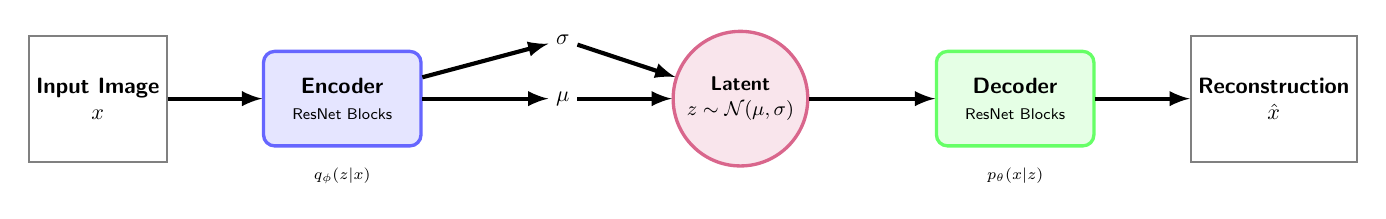
\begin{tikzpicture}[
    node distance=2cm,
    auto,
    scale=0.8,
    transform shape,
    box/.style={rectangle, rounded corners, minimum width=2.5cm, minimum height=1.5cm, align=center, draw=black!70, very thick, font=\sffamily},
    enc/.style={box, fill=blue!10, draw=blue!60},
    dec/.style={box, fill=green!10, draw=green!60},
    latent/.style={circle, minimum size=1.5cm, align=center, draw=purple!60, fill=purple!10, very thick, font=\sffamily\small},
    image/.style={rectangle, minimum size=2cm, align=center, draw=black!50, fill=white, thick, font=\sffamily},
    arrow/.style={-latex, thick, line width=1.5pt}
]

    % Input Image
    \node[image] (input) {\textbf{Input Image}\\$x$};

    % Encoder
    \node[enc, right=1.5cm of input] (encoder) {\textbf{Encoder}\\\scriptsize ResNet Blocks};
    
    % Latent Distribution
    \node[right=2cm of encoder] (mu) {$\mu$};
    \node[above=0.5cm of mu] (sigma) {$\sigma$};
    \node[latent, right=1.5cm of mu] (z) {\textbf{Latent}\\$z \sim \mathcal{N}(\mu, \sigma)$};
    
    % Decoder
    \node[dec, right=2cm of z] (decoder) {\textbf{Decoder}\\\scriptsize ResNet Blocks};
    
    % Output Image
    \node[image, right=1.5cm of decoder] (output) {\textbf{Reconstruction}\\$\hat{x}$};

    % Connections
    \draw[arrow] (input) -- (encoder);
    \draw[arrow] (encoder) -- node[above] {} (mu);
    \draw[arrow] (encoder) -- (sigma);
    \draw[arrow] (mu) -- (z);
    \draw[arrow] (sigma) -- (z);
    \draw[arrow] (z) -- (decoder);
    \draw[arrow] (decoder) -- (output);
    
    % Annotations
    \node[below=0.2cm of encoder] {\scriptsize $q_\phi(z|x)$};
    \node[below=0.2cm of decoder] {\scriptsize $p_\theta(x|z)$};

\end{tikzpicture}
\end{document}
